\documentclass[10pt,english,a4paper]{report}

\usepackage[utf8]{inputenc}
\usepackage[english]{babel}

\usepackage[T1]{fontenc}
\usepackage{times}
% \usepackage{needspace}
\usepackage{parskip}
\usepackage[a4paper,top=8mm,bottom=15mm,left=15mm,right=15mm,includeheadfoot,headheight=5mm,headsep=5mm,footskip=10mm]{geometry}

\usepackage{fancyhdr}
\pagestyle{fancy}
\renewcommand\rfoot{
	\hfill \thepage
}
\renewcommand\lfoot{
	\hfill \thepage
}

\usepackage[pdftex]{graphicx}
\usepackage[pdftex,hidelinks]{hyperref}
\usepackage{tikz}
\usepackage{ifthen}
\usetikzlibrary{shapes,arrows,calc,patterns,backgrounds,fit}

\tikzstyle{block} = [draw, text=white!90!gray, fill=blue!20!gray, rectangle, rounded corners, minimum height=2.6em, minimum width=5.5em]
\tikzstyle{sum} = [draw, fill=blue!20, circle, node distance=1cm]
\tikzstyle{input} = [coordinate]
\tikzstyle{output} = [coordinate]
\tikzstyle{pinstyle} = [pin edge={to-,thin,black}]
\tikzstyle{bus} = [thick,double distance=0.1em,>=latex']
\tikzstyle{secnsecreg}=[minimum width=13em,minimum height=2em]
\tikzstyle{secure}=[secnsecreg,fill=blue!50!gray,fill opacity=0.8]
\tikzstyle{nonsecure}=[secnsecreg,fill opacity=0.6,fill=orange]
\tikzstyle{sg}=[secnsecreg,pattern=crosshatch,pattern color=blue!50!gray,fill opacity=0.8]

\colorlet{ltb_green}{green!70!black}
\colorlet{ltb_blue}{blue!75!black}
\colorlet{ltb_orange}{orange!80}
\colorlet{ltb_yellow}{yellow!65!orange}
\colorlet{ltb_red}{red!80!black}
\colorlet{ltb_highlight_red}{ltb_red}
\colorlet{ltb_highlight_orange}{ltb_orange}
\tikzstyle{ltb_blue_trans}=[fill=blue!25,fill opacity=0.5]
\tikzstyle{ltb_orange_trans}=[fill opacity=0.5,fill=orange]

\makeatletter
\@ifclassloaded{beamer}{
    \newcommand{\ltbbeamer}[0]{1=1}
}{
    \newcommand{\ltbbeamer}[0]{1=0}
}
\makeatother
\newcommand{\mytikzrefnode}[1]{\tikz[remember picture,baseline=-.5ex] \coordinate (#1) {};}

\tikzstyle{every picture}+=[remember picture]

\pdfminorversion=5  % PDF 1.5 (Acrobat 5.x)
\pdfcompresslevel=1 % [0..9], 0: no compression, 9: strong compression
\pdfimageresolution=300

\usepackage{nameref}
\usepackage{listings}
\lstset{frame=tb,
  language=C,
  aboveskip=3mm,
  belowskip=3mm,
  showstringspaces=false,
  columns=flexible,
  basicstyle={\small\ttfamily},
  numbers=none,
  numberstyle=\tiny,
  breaklines=true,
  breakatwhitespace=true,
  tabsize=4
}
\newcommand{\gitdate}{__GITDATE__}


\begin{document}
\pagenumbering{roman}

\begin{center}
	\vspace*{1.5\baselineskip}
	\large
	\textbf{\huge Documentation for JTAG Switcher}\\
	\vspace{1.5\baselineskip}
	{\gitdate}\\
	\vspace{10\baselineskip}
	\LARGE
	\textbf{License}\\
\end{center}
\textbf{The MIT License}

Copyright (c) 2018-2019 Lauterbach GmbH, Ingo Rohloff\\

Permission is hereby granted, free of charge,
to any person obtaining a copy of this software and
associated documentation files (the "Software"), to
deal in the Software without restriction, including
without limitation the rights to use, copy, modify,
merge, publish, distribute, sublicense, and/or sell
copies of the Software, and to permit persons to whom
the Software is furnished to do so,
subject to the following conditions:

The above copyright notice and this permission notice
shall be included in all copies or substantial portions of the Software.

THE SOFTWARE IS PROVIDED "AS IS", WITHOUT WARRANTY OF ANY KIND,
EXPRESS OR IMPLIED, INCLUDING BUT NOT LIMITED TO THE WARRANTIES
OF MERCHANTABILITY, FITNESS FOR A PARTICULAR PURPOSE AND NONINFRINGEMENT.
IN NO EVENT SHALL THE AUTHORS OR COPYRIGHT HOLDERS BE LIABLE FOR
ANY CLAIM, DAMAGES OR OTHER LIABILITY, WHETHER IN AN ACTION OF CONTRACT,
TORT OR OTHERWISE, ARISING FROM, OUT OF OR IN CONNECTION WITH THE
SOFTWARE OR THE USE OR OTHER DEALINGS IN THE SOFTWARE.

\cleardoublepage
\pagenumbering{arabic}

\setcounter{tocdepth}{10}
\renewcommand\contentsname{Table of Contents}
\tableofcontents

\chapter{Introduction}
Lauterbach has published the VHDL source code of the JTAG Switcher component at:\\
{\tt https://www.lauterbach.com/jtag\_switcher.html}

\section{IEEE 1149.1 aka JTAG}
The IEEE standard 1149.1 defines a physical interface to an integrated circuit (IC).

This interface allows a suitable tool to exchange data with circuitry inside the IC.
This interface was originally intended for testing assembled printed circuit boards (PCBs).

Nowadays this interface is used as a general purpose testing and debugging interface,
allowing a suitable tool to communicate with various debug logic included in an IC.

\newpage
\section{JTAG overview}
\label{jtagintro}

A JTAG interface consists of four mandatory and one optional signal. These are:
\begin{itemize}
\item TCK : Test Clock, clocks all D-flip-flops, which are part of the JTAG architecture.
\item TMS : Test Machine State, controls the JTAG TAP Controller state machine
\item TDI : Test Data In, serial data send into the JTAG architecture.
\item TDO : Test Data Out, serial data received from the JTAG architecture.
\item TRST* : Test Reset, optional reset signal, which will {\em asynchronously} reset the JTAG TAP Controller state machine,
putting it into the "Test-Logic-Reset" state.
\end{itemize}
These four (or five) signals grouped together are called Test Access Port (TAP).

These four signals connect to the internal JTAG architecture. The overall
architecture looks like this (TRST* is excluded here).
\begin{center}
	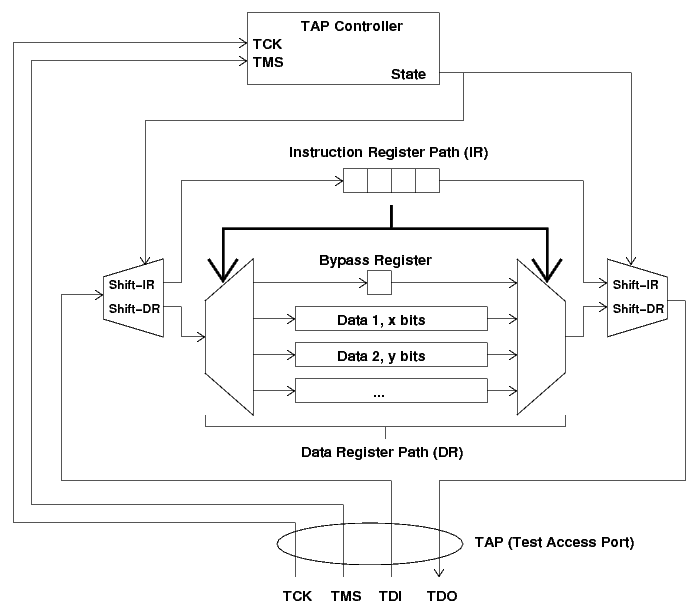
\includegraphics[width=0.8\textwidth]{jtag_logic.png}
\end{center}
Details:

The {\tt Instruction Register} (IR) shift path is accessed, when the TAP Controller is in the {\tt Shift-IR} state.

The {\tt Data Register} (DR) shift path is accessed, when the TAP Controller is in the {\tt Shift-DR} state.

In all other states (all except {\tt Shift-DR} and {\tt Shift-IR}) the data coming in from TDI should be ignored and TDO should be tristated.

The IR should have a fixed length. The content of the IR defines which DR shift path is accessed in the Shift-DR state.

The 1149.1 IEEE standard defines that a device {\em must} support the BYPASS instruction; this instruction has to have a code/value of all ones (so 1111...).
If the IR contains the BYPASS instruction the shift path in the Shift-DR state {\em must} access the bypass register.

\newpage
The TAP Controller is a state machine, which changes state at each
rising edge of TCK. The state progression is controlled via
the value of the TMS signal which is sampled on a rising edge of TCK.

The state machine has sixteen states and behaves as described in the
following diagram.
\begin{center}
	\includegraphics[width=0.8\textwidth]{jtag_machine.png}
\end{center}
The sixteen states are abbreviated in the above picture. They are called:
\begin{tabbing}
State Column mm \= Abbrev \= State Colxxxxxx \= Abbrevxxx \= State Colxxxxxx \= Abbrevxxx \kill
Test-Logic-Reset \> (TLR) \> Select-DR-Scan  \> (SelDR) \> Select-IR-Scan  \> (SelIR) \\
Run-Test/Idle    \> (RTI) \> Capture-DR      \> (CapDR) \> Capture-IR      \> (CapIR) \\
                 \>       \> Shift-DR        \> (ShfDR) \> Shift-IR        \> (ShfIR) \\
                 \>       \> Exit1-DR        \> (Ex1DR) \> Exit1-IR        \> (Ex1IR) \\
                 \>       \> Pause-DR        \> (PsDR)  \> Pause-IR        \> (PsIR)  \\
                 \>       \> Exit2-DR        \> (Ex2DR) \> Exit2-IR        \> (Ex2IR) \\
                 \>       \> Update-DR       \> (UpdDR) \> Update-IR       \> (UpdIR) \\
\end{tabbing}

As an example, here is a waveform diagram, which shows an access to a three-bit DR.
The TAP controller state sequence starts and ends in the Run-Test/Idle state.
\begin{center}
	\includegraphics[width=\textwidth]{jtag_shift_example.png}
\end{center}

\newpage
\section{JTAG chaining}
If you have several ICs on a PCB and each of these ICs has a JTAG TAP (JTAG Test Access Port), JTAG allows you
to daisy chain the TAPs in the following manner (the following diagram shows three ICs connected to one PCB wide TAP):
\begin{center}
%	\includegraphics[width=0.8\textwidth]{jtag_chain_01.png}
	\newcommand{\jtag}[2]
{
\node [jnode,anchor=west] (jtag#1) at #2 {};
\node [right] at ([yshift=0.5em]jtag#1.west) (_jtag#1_tdi) {TDI};
\node [left] at ([yshift=0.5em]jtag#1.east) (_jtag#1_tdo) {TDO};
\node [above] at ([xshift=-1.5em]jtag#1.south) (_jtag#1_tck)  {TCK};
\node [above] at ([xshift=1.5em]jtag#1.south) (_jtag#1_tms) {TMS};
\coordinate (jtag#1_tdi) at (_jtag#1_tdi.west);
\coordinate (jtag#1_tdo) at (_jtag#1_tdo.east);
\coordinate (jtag#1_tck) at (_jtag#1_tck.south);
\coordinate (jtag#1_tms) at (_jtag#1_tms.south);
}
\tikzstyle{jnode}=[draw,rounded corners,minimum height=3.5em,minimum width=8em]
\tikzstyle{buffer}=[draw=black,fill=white,regular polygon,regular polygon sides=3,rotate=30,inner sep=0,minimum height=1.5em]

\tikzstyle{demux} = [trapezium,draw,shape border rotate=90,trapezium stretches body]
\tikzstyle{mux} = [trapezium,draw,shape border rotate=270,trapezium stretches body]

\begin{tikzpicture}[]
\jtag{1}{(0,0)}
\jtag{2}{([xshift=3em]jtag1.east)}
\jtag{3}{([xshift=3em]jtag2.east)}

\path (jtag1_tck) to ++(0,-1.5em) coordinate (tck_inters) -- ++(0,-3.5em) coordinate (tck_in);
\path (jtag1_tms) to ++(0,-2.5em) coordinate (tms_inters) -- (tck_in -| jtag1_tms) coordinate (tms_in);
\coordinate (tdi_in) at ($(tms_in)!2!(tck_in)$);
\coordinate (tdo_in) at ($(tck_in)!2!(tms_in)$);

\node [below] at (tdi_in) {TDI};
\node [below] at (tck_in) {TCK};
\node [below] at (tms_in) {TMS};
\node [below] at (tdo_in) {TDO};

\draw [->,thick] (jtag1_tdo) -- (jtag2_tdi);
\draw [->,thick] (jtag2_tdo) -- (jtag3_tdi);

\draw [<-,thick] (jtag1_tdi) -| ([xshift=-1.5em]jtag1.south west) -- +(0,-3.5em) -| (tdi_in);
\draw [->,thick] (jtag3_tdo) -|  ([xshift=1.5em]jtag3.south east) -- +(0,-3.5em) -| (tdo_in);
\draw [->,thick] (tck_in) -- (jtag1_tck);
\draw [->,thick] (tms_in) -- (jtag1_tms);
\draw [fill] (tms_inters) circle (0.15em);
\draw [fill] (tck_inters) circle (0.15em);
\draw [->,thick] (tck_inters) -| (jtag2_tck);
\draw [->,thick] (tck_inters) -| (jtag3_tck);
\draw [->,thick] (tms_inters) -| (jtag2_tms);
\draw [->,thick] (tms_inters) -| (jtag3_tms);

\end{tikzpicture}
\end{center}
TCK and TMS are routed in a star fashion from the PCB TAP to each of the IC TAPs.

TDI and TDO are chained so that the TDO of one IC TAP is routed to the TDI of the next IC TAP.

With this approach, the IR and DR shift paths are chained together.
This means that you access all IRs and all DRs at once when executing a shift TAP controller state sequence.

The usual approach to communicate with one TAP is to load BYPASS
instructions into the IRs of all other TAPs. When you then execute a DR shift
TAP controller state sequence, you will have to receive and send some additional
bits to account for the BYPASS registers of the additional TAPs, but this is not
a big problem. In such a scenario you only have to know how many bits precede
and follow the real instruction bits of the TAP you want to access and how many
extra bits you have to shift before and after the DR data. So basically you only
need four values which define how to access the TAP you want. These four values
are:
\begin{itemize}
\item {\tt IRPRE} : Number of '1' bits to shift before the IR bits.
\item {\tt IRPOST} : Number of '1' bits to shift after the IR bits.
\item {\tt DRPRE} : Number of BYPASS registers before the DR.
\item {\tt DRPOST} : Number of BYPASS registers after the DR.
\end{itemize}

The following picture tries to illustrate how that works. In this example the middle TAP is accessed.
\begin{center}
	\includegraphics[width=0.9\textwidth]{jtag_chain_prepost.png}
\end{center}

\chapter{JTAG Switcher overview}
\section{Motivation}
When trying to chain several ICs together into a JTAG chain there are various potential problems.

Two of the most common ones are:
\begin{itemize}
\item Different signaling levels
\item TDI to TDO chain might become non-functional in a single IC, which will break the {\em whole} JTAG chain.
\end{itemize}

Here is a picture illustrating these problems:
\begin{center}
	%\includegraphics[width=0.8\textwidth]{jtag_chain_broken.png}
	\newcommand{\jtag}[2]
{
\node [jnode,anchor=west] (jtag#1) at #2 {};
\node [right] at ([yshift=0.5em]jtag#1.west) (_jtag#1_tdi) {TDI};
\node [left] at ([yshift=0.5em]jtag#1.east) (_jtag#1_tdo) {TDO};
\node [above] at ([xshift=-1.5em]jtag#1.south) (_jtag#1_tck)  {TCK};
\node [above] at ([xshift=1.5em]jtag#1.south) (_jtag#1_tms) {TMS};
\coordinate (jtag#1_tdi) at (_jtag#1_tdi.west);
\coordinate (jtag#1_tdo) at (_jtag#1_tdo.east);
\coordinate (jtag#1_tck) at (_jtag#1_tck.south);
\coordinate (jtag#1_tms) at (_jtag#1_tms.south);
}
\tikzstyle{jnode}=[draw,rounded corners,minimum height=3.5em,minimum width=8em]
\tikzstyle{buffer}=[draw=black,fill=white,regular polygon,regular polygon sides=3,rotate=30,inner sep=0,minimum height=1.5em]

\tikzstyle{demux} = [trapezium,draw,shape border rotate=90,trapezium stretches body]
\tikzstyle{mux} = [trapezium,draw,shape border rotate=270,trapezium stretches body]

\begin{tikzpicture}[inner frame sep=0]
%\begin{tikzpicture}[show background rectangle,inner frame sep=0]
\jtag{1}{(0,0)}
\jtag{2}{([xshift=3em]jtag1.east)}
\jtag{3}{([xshift=3em]jtag2.east)}

\path (jtag1_tck) to ++(0,-1.5em) coordinate (tck_inters) -- ++(0,-3.5em) coordinate (tck_in);
\path (jtag1_tms) to ++(0,-2.5em) coordinate (tms_inters) -- (tck_in -| jtag1_tms) coordinate (tms_in);
\coordinate (tdi_in) at ($(tms_in)!2!(tck_in)$);
\coordinate (tdo_in) at ($(tck_in)!2!(tms_in)$);

\node [below] at (tdi_in) {TDI};
\node [below] at (tck_in) {TCK};
\node [below] at (tms_in) {TMS};
\node [below] at (tdo_in) {TDO};

\draw [->,thick] (jtag1_tdo) -- node [buffer] {} (jtag2_tdi);
\draw [->,thick] (jtag2_tdo) -- node [buffer] {} (jtag3_tdi);

\draw [<-,thick] (jtag1_tdi) -| ([xshift=-1.5em]jtag1.south west) -- +(0,-2.5em) -| (tdi_in);
\draw [->,thick] (jtag3_tdo) -|  ([xshift=1.5em]jtag3.south east) -- +(0,-2.5em) -| (tdo_in);
%\draw [->,thick] (tck_in) -- (jtag1_tck);
\draw [->,thick] (tck_in) -- ++(0,.6em) node [draw,minimum height=2em,minimum width=2em,anchor=south,fill=white] (tck_buf) {};
\draw [<-,thick] ($(tck_buf.south west)!0.25!(tck_buf.south east)$) -- +(0,-0.35em) -| (tck_in);
\draw [<-,thick] ($(tck_buf.south west)!0.75!(tck_buf.south east)$) -- +(0,-0.35em) -| (tck_in);
\coordinate (tck_buf_out1) at ($(tck_buf.north west)!0.25!(tck_buf.north east)$);
\coordinate (tck_buf_out2) at ($(tck_buf.north west)!0.5!(tck_buf.north east)$);
\coordinate (tck_buf_out3) at ($(tck_buf.north west)!0.75!(tck_buf.north east)$);
\node [buffer] at (tck_buf) {};

\draw [->,thick] (tms_in) -- ++(0,.6em) node [draw,minimum height=2em,minimum width=2em,anchor=south,fill=white] (tms_buf) {};
\draw [<-,thick] ($(tms_buf.south west)!0.25!(tms_buf.south east)$) -- +(0,-0.35em) -| (tms_in);
\draw [<-,thick] ($(tms_buf.south west)!0.75!(tms_buf.south east)$) -- +(0,-0.35em) -| (tms_in);
\coordinate (tms_buf_out1) at ($(tms_buf.north west)!0.25!(tms_buf.north east)$);
\coordinate (tms_buf_out2) at ($(tms_buf.north west)!0.5!(tms_buf.north east)$);
\coordinate (tms_buf_out3) at ($(tms_buf.north west)!0.75!(tms_buf.north east)$);
\node [buffer] at (tms_buf) {};

\draw [thick,->] (tck_buf_out1) edge [->] ++(0,0.35em) |- (tck_buf_out1 |- jtag1_tck);
\draw [thick,->] (tck_buf_out2) edge [->] ++(0,0.35em) ++(0,0.35em) |- ([yshift=-0.6em]jtag2_tck) -- (jtag2_tck);
\draw [thick,->] (tck_buf_out3) edge [->] ++(0,0.35em) ++(0,0.35em) |- ([yshift=-0.8em]jtag3_tck) -- (jtag3_tck);
\draw [thick,->] (tms_buf_out1) edge [->] ++(0,0.35em) |- (tms_buf_out1 |- jtag1_tms);
\draw [thick,->] (tms_buf_out2) edge [->] ++(0,0.35em) ++(0,0.35em) |- ([yshift=-1.2em]jtag2_tms) -- (jtag2_tms);
\draw [thick,->] (tms_buf_out3) edge [->] ++(0,0.35em) ++(0,0.35em) |- ([yshift=-1.4em]jtag3_tms) -- (jtag3_tms);

\path (tdi_in) |- node [thick,buffer,rotate=-30,yshift=-0.1em] (tdi_in_buf) {} (tck_buf.west);
\path (tdo_in) |- node [thick,buffer,rotate=30] (tdo_in_buf) {} (tck_buf.west);

\ifthenelse{\ltbbeamer}{
	\node [draw=ltb_red,rounded corners,fit=(jtag1),label={\tiny{}VREF=?V}] {};
	\node [draw=ltb_blue,rounded corners,fit=(jtag2),label={\tiny{}VREF=?V}] {};
	\node [draw=ltb_green,rounded corners,fit=(jtag3),label={\tiny{}VREF=?V}] {};
}{
	\node [fit=(jtag1),label={\tiny{}IC 1 - $VREF_1$}] {};
	\node [fit=(jtag2),label={\tiny{}IC 2 - $VREF_2$}] {};
	\node [fit=(jtag3),label={\tiny{}IC 3 - $VREF_3$}] {};
}
\begin{scope}[on background layer]
	\draw [dashed,gray] ([xshift=-4em]tck_buf.west) -- (tck_buf.west -| tdo_in_buf) -- +(2em,0) node [below,xshift=1em] {\tiny{}VREF=?V};
\end{scope}
\end{tikzpicture}
	\begin{tikzpicture}[overlay]
		\draw [draw,thick,ltb_red,shorten >=-1em,shorten <=-1em] (jtag2.south west) -- (jtag2.north east);
		\draw [draw,thick,ltb_red,shorten >=-1em,shorten <=-1em] (jtag2.south east) -- (jtag2.north west);
	\end{tikzpicture}
\end{center}
In the situation depicted above, you might circumvent the different signaling voltage levels
by including appropriate dual-voltage buffers.

But if additionally {\tt IC 2} is sometimes powered, sometimes not, the chain will be broken
once {\tt IC 2} is unpowered, making it impossible to access {\tt IC 1} and {\tt IC 3}.

\newpage
The "JTAG Switcher" implements a solution for these problems.

The idea is to use an FPGA as buffer between the PCB TAP and the different TAPs of the ICs,
like this:
\begin{center}
	%\includegraphics[width=0.8\textwidth]{jtag_jswitch_1.png}
	\newcommand{\jtag}[2]
{
\node [jnode,anchor=west] (jtag#1) at #2 {};
\node [right] at ([yshift=0.5em]jtag#1.west) (_jtag#1_tdi) {TDI};
\node [left] at ([yshift=0.5em]jtag#1.east) (_jtag#1_tdo) {TDO};
\node [above] at ([xshift=-1.5em]jtag#1.south) (_jtag#1_tck)  {TCK};
\node [above] at ([xshift=1.5em]jtag#1.south) (_jtag#1_tms) {TMS};
\coordinate (jtag#1_tdi) at (_jtag#1_tdi.west);
\coordinate (jtag#1_tdo) at (_jtag#1_tdo.east);
\coordinate (jtag#1_tck) at (_jtag#1_tck.south);
\coordinate (jtag#1_tms) at (_jtag#1_tms.south);
}
\tikzstyle{jnode}=[draw,rounded corners,minimum height=3.5em,minimum width=8em]
\tikzstyle{buffer}=[draw=black,fill=white,regular polygon,regular polygon sides=3,rotate=30,inner sep=0,minimum height=1.5em]

\tikzstyle{demux} = [trapezium,draw,shape border rotate=90,trapezium stretches body]
\tikzstyle{mux} = [trapezium,draw,shape border rotate=270,trapezium stretches body]

\begin{tikzpicture}[]
\jtag{1}{(0,0)}
\jtag{2}{([xshift=3em]jtag1.east)}
\jtag{3}{([xshift=3em]jtag2.east)}

\draw ($(jtag1.south west)+(-1.5em,-1.5em)$) coordinate (fpga_north_west) -- ($(jtag3.south east)+(1.5em,-1.5em)$) coordinate (fpga_north_east);
\draw (fpga_north_west) -- +(0,-4em) coordinate (fpga_south_west);
\draw (fpga_north_east) -- (fpga_north_east |- fpga_south_west) coordinate (fpga_south_east); 
\draw (fpga_south_west) -- coordinate (fpga_south) (fpga_south_east);
\node [anchor=south west] at (fpga_south_west) {PCB TAP};
\node [anchor=south east] at (fpga_south_east) {JTAG Switcher FPGA};

\coordinate (fpga_tck_in) at ([xshift=-1.3em]fpga_south);
\coordinate (fpga_tms_in) at ($(fpga_tck_in)!2!(fpga_south)$);
\coordinate (fpga_tdi_in) at ($(fpga_tms_in)!2!(fpga_tck_in)$);
\coordinate (fpga_tdo_out) at ($(fpga_tck_in)!2!(fpga_tms_in)$);

\draw ([xshift=-0.5em]fpga_tdi_in) coordinate (iobank3_vccio) -- ++(0,1.5em) -| ([xshift=0.5em]fpga_tdo_out) node [yshift=0.3em,anchor=base east] {\tiny{IO-Bank}};

\draw [<-,thick] (fpga_tck_in) -- +(0,-1.2em) coordinate (tck_in) node [below] {TCK};
\draw [<-,thick] (fpga_tms_in) -- (fpga_tms_in |- tck_in) node [below] {TMS};
\draw [<-,thick] (fpga_tdi_in) -- (fpga_tdi_in |- tck_in) node [below] {TDI};
\draw [->,thick] (fpga_tdo_out) -- (fpga_tdo_out |- tck_in) node [below] {TDO};

\draw [thick] (jtag1_tdo) -| ([xshift=0.5em]jtag1_tdo |- fpga_north_west) coordinate (iobank1_tdo);
\draw [thick] (jtag1_tdi) -| ([xshift=-0.5em]jtag1_tdi |- fpga_north_west) coordinate (iobank1_tdi);
\draw [thick] (jtag1_tms) -- (jtag1_tms |- fpga_north_west);
\draw [thick] (jtag1_tck) -- (jtag1_tck |- fpga_north_west);
\draw ([xshift=-0.5em]iobank1_tdi) -- ++(0,-1.5em) coordinate (iobank1_vccio) -| node [yshift=0.3em,anchor=base east] {\tiny{IO-Bank}} ([xshift=0.5em]iobank1_tdo);

\draw [thick] (jtag2_tdo) -| ([xshift=0.5em]jtag2_tdo |- fpga_north_west) coordinate (iobank2_tdo);
\draw [thick] (jtag2_tdi) -| ([xshift=-0.5em]jtag2_tdi |- fpga_north_west) coordinate (iobank2_tdi);
\draw [thick] (jtag2_tms) -- (jtag2_tms |- fpga_north_west);
\draw [thick] (jtag2_tck) -- (jtag2_tck |- fpga_north_west);
\draw ([xshift=-0.5em]iobank2_tdi) -- ++(0,-1.5em) coordinate (iobank2_vccio) -| node [yshift=0.3em,anchor=base east] {\tiny{IO-Bank}} ([xshift=0.5em]iobank2_tdo);

\draw [thick] (jtag3_tdo) -| ([xshift=0.5em]jtag3_tdo |- fpga_north_west) coordinate (iobank3_tdo);
\draw [thick] (jtag3_tdi) -| ([xshift=-0.5em]jtag3_tdi |- fpga_north_west) coordinate (iobank3_tdi);
\draw [thick] (jtag3_tms) -- (jtag3_tms |- fpga_north_west);
\draw [thick] (jtag3_tck) -- (jtag3_tck |- fpga_north_west);
\draw ([xshift=-0.5em]iobank3_tdi) -- ++(0,-1.5em) coordinate (iobank3_vccio) -| node [yshift=0.3em,anchor=base east] {\tiny{IO-Bank}} ([xshift=0.5em]iobank3_tdo);

\node [fit=(jtag1),label={\tiny{}IC 1 - $VREF_1$}] {};
\node [fit=(jtag2),label={\tiny{}IC 2 - $VREF_2$}] {};
\node [fit=(jtag3),label={\tiny{}IC 3 - $VREF_3$}] {};

\node [yshift=0.3em,anchor=base west] at (iobank1_vccio) {\tiny{}$VCC_{IO}=VREF_1$};
\node [yshift=0.3em,anchor=base west] at (iobank2_vccio) {\tiny{}$VCC_{IO}=VREF_2$};
\node [yshift=0.3em,anchor=base west] at (iobank3_vccio) {\tiny{}$VCC_{IO}=VREF_3$};

\end{tikzpicture}
\end{center}
The JTAG Switcher has two main functions:
\begin {itemize}
\item The JTAG Switcher translates to the appropriate voltage levels.
\item The JTAG Switcher can modify which TAPs are visible on the PCB TAP.
So it provides the ability to choose which TAPs are included in the JTAG chain.
\end{itemize}

\newpage
\section{Basic circuitry}
Here is an overview of the internal circuitry of the JTAG Switcher FPGA.
In this example three JTAG slave TAPs are connected to the FPGA.
In general the number of JTAG slave TAPs is configurable.
\begin{center}
	\includegraphics[width=0.8\textwidth]{jtag_jswitch_arch_2.png}
\end{center}
Explanations:
\begin{itemize}
\item The "JTAG Switcher internal control logic" is responsible for controlling
three control bits: {\tt EN1}, {\tt EN2}, {\tt EN3}.
\item A JTAG slave TAP is completely excluded from the JTAG chain
if the corresponding {\tt ENx} bit is '0'. Exclusion from the JTAG chain means:
\begin{itemize}
\item TDI to this JTAG slave TAP is tri-stated.
\item TCK to this JTAG slave TAP is gated and kept at value '0'.
\item TMS to this JTAG slave TAP is kept at value '1'.
\item TDO from this JTAG slave TAP is ignored.
\end{itemize}
\item When all {\tt ENx} bits are '0', no JTAG slave TAP is visible on the PCB TAP.
In this case {\em only} the "JTAG Switcher internal control logic" is visible
on the PCB TAP.
\end{itemize}

\newpage
\section{Design decisions}
\subsection{JTAG Switcher should conform to IEEE 1149.1}
The JTAG Switcher internal logic should behave like a IEEE 1149.1 TAP.

Rationale:
\begin{itemize}
\item Configuration of the JTAG Switcher does not require any extra pins.
\item Regular JTAG tools are easily able to just ignore the JTAG Switcher, so
these tools do not need to have any knowledge of the internal logic of the JTAG Switcher.
\end{itemize}

\subsection{Transparency}
You might configure the JTAG Switcher once. The JTAG Switcher {\em will not}
modify the selected JTAG slave TAPs because of entering the Test-Logic-Reset state
or because of assertion of the TRST* signal.

Rationale:
\begin{itemize}
\item Once the JTAG Switcher is configured, a JTAG tool does not need to know
how the JTAG Switcher behaves internally. All JTAG TAP Controller state sequences
are allowed.
\item This makes the JTAG Switcher transparent to a JTAG tool; the configuration
stays stable and the JTAG Switcher will act like an inert extra TAP on the JTAG chain.
\end{itemize}

\subsection{First in JTAG chain}
The JTAG Switcher internal logic is directly connected to the TDI signal of
the PCB TAP. So the JTAG Switcher internal logic always appears to be the "first" device
in the JTAG chain.

Rationale:
\begin{itemize}
\item This construction will always allow recovery if the JTAG chain is broken
by an inaccessible JTAG slave TAP: Since the JTAG Switcher will still be directly connected to TDI,
a series of {\em write} accesses to the JTAG Switcher internal logic IR and DR shift paths is possible.
This way arbitrary commands can still be sent to the JTAG Switcher internal logic and thus
allow for the exclusion of all JTAG slave TAPs from the JTAG Chain, putting the JTAG Chain back into
a usable state.
\end{itemize}

\subsection{JTAG slave TCK clock gating}
JTAG slave TAPs which are not selected, will see no toggling on the corresponding JTAG slave TCK signal.

Rationale:
\begin{itemize}
\item Some ICs exhibit JTAG TAPs, which produce side effects, if TCK toggles.
By keeping the TCK signal of an excluded JTAG slave TAP stable, all these side effects are avoided.
\end{itemize}

\subsection{Change selection {\em only} in the Run-Test/Idle JTAG TAP Controller state}
The JTAG Switcher will change the value of the {\tt ENx} bits,
which control the in- and exclusion of JTAG slave TAPs {\em only} in the Run-Test/Idle JTAG
TAP Controller state.

Rationale:
\begin{itemize}
\item A JTAG slave TAP is always ex- and included onto the JTAG TAP chain while the
TAP Controller state is in Run-Test/Idle. With this construction all excluded
JTAG slave TAP Controllers are kept in the Run-Test/Idle state. This way there is one
consistent state for all excluded TAP Controllers.
\item This allows a series of DR and IR shift path accesses to the JTAG Switcher control
logic, while then still modifying the selection of {\em all} JTAG slave TAPs at exactly the same
TCK clock edge: As long as the Run-Test/Idle state is not reached the selection will not change.
Only by entering the Run-Test/Idle state the configured selection will get activated.
\end{itemize}

\chapter{JTAG Switcher implementation}
This section tries to describe the architecture and behavior of the
"JTAG Switcher internal control logic". This logic is responsible
for implementing access to all control registers.

\section{JTAG to bus access translation}
Internally the JTAG Switcher uses a very simple 16-bit wide data bus.
This bus behaves similarly to any other known peripheral buses: So a
bus master drives:
\begin{itemize}
\item An Address to all bus slaves.
\item A 16-bit wide data word to all bus slaves.
\item A write strobe (asserted for one TCK clock cycle)
\item A read strobe (asserted for one TCK clock cycle)
\end{itemize}

The bits in the 16-bit wide data word are numbered from 0 to 15.

Bit 0 corresponds to the least significant bit ($2^0$).

Bit 15 corresponds to the most significant bit ($2^{15}$).

The function of the bus master is to translate JTAG accesses to
bus accesses on the internal bus. The basic operations supported are:
\begin{itemize}
\item Set address for bus access
\item Write to bus
\item Read from bus
\item Read from and write to bus
\item Set address and write to bus
\end{itemize}
All these operations are executed via a DR Shift Sequence.

Read operations are triggered by the Capture-DR state.

Write operations and setting the address are triggered by the Update-DR state.

The content of the IR defines which operation is currently selected.

\newpage
Example Sequences:

{\bf Set bus address and then write a 16 bit value to this address}
\begin{itemize}
\item Shift "Set Address" instruction into IR of JTAG Switcher.
\item Shift address for bus access into DR of JTAG Switcher.
\item Shift "Write to bus" instruction into IR of JTAG Switcher.
\item Shift 16-bit value (via TDI) into DR of JTAG Switcher.
\end{itemize}

{\bf Set bus address and then read a 16 bit value from this address}
\begin{itemize}
\item Shift "Set Address" instruction into IR of JTAG Switcher.
\item Shift address for bus access into DR of JTAG Switcher.
\item Shift "Read from bus" instruction into IR of JTAG Switcher.
\item Shift out 16-bit value (via TDO) from DR of JTAG Switcher.
\end{itemize}

{\bf Combined: Set bus address and write a 16 bit value to this address}

This operation is implemented for more efficient access to modify
control bits.
\begin{itemize}
\item Shift "Set address and write to bus" instruction into IR of JTAG Switcher.
\item Shift address + 16-bit value for bus access into DR of JTAG Switcher.
\end{itemize}

\section{Set and Clear control bit accesses}
Control bits inside the JTAG Switcher use the concept of "Set and Clear" bits
for modification.

To modify control bits a 16-bit write access to the bus will be used
to modify up to 8 control bits.

Each control bit reacts to two bits of the 16-bit data word. The four possible
combinations for the two bits of the 16-bit data word are interpreted in the
following manner:
\begin{itemize}
\item {\tt 00}: "No Operation"; the corresponding control bit is {\em not} modified
\item {\tt 01}: "Set Bit"; the corresponding control bit is set to '1'.
\item {\tt 10}: "Clear Bit"; the corresponding control bit is set to '0'.
\item {\tt 11}: "Clear Bit"; the corresponding control bit is set to '0'.
\end{itemize}

For consistency the JTAG Switcher uses a fixed mapping from bits of a
16-bit data word to modify up to 8 control bits:
\begin{tabbing}
mmmmmmmmmmm\= mmmmm \= mmmmm \= mmmmm \= mmmmm \= mmmmm \= mmmmm \= mmmmm \= mmmmm \kill
Data Bits   \> 15..14 \> 13..12 \> 11..10 \> 9..8 \> 7..6 \> 5..4 \> 3..2 \> 1..0 \\
Slave TAP Nr\>      8 \>    7   \>      6 \>    5 \>    4 \>    3 \>    2 \>    1 \\
\end{tabbing}

All even numbered bits of a 16-bit data word (0, 2, 4, 6, 8, 10, 12, 14) are used
to indicate "Set Bit" operations. All odd numbered bits of a 16-bit data word
(1, 3, 5, 7, 9, 11, 13, 15) are used to indicate "Clear Bit" operations.
"Clear Bit" operations have a higher priority, so if both
"Set Bit" and "Clear Bit" are set, a "Clear Bit" operation is performed.

A read access to a 16-bit data word will output the value of the corresponding control bits
on the even numbered bits of the 16-bit data word.

Rationale:

This scheme allows to modify single control bits without knowledge of any other control bits.
Without the "Set/Clear" scheme, you usually would have to read out all control bits
accessed via one specific data word, then mask or set the control bits you want to modify and
then to write back the resulting value.

With the "Set/Clear" scheme you do not need to know any values of control bits to modify
a single control bit: You write the operation you need ({\tt 01} or {\tt 10}) for the
control bits you want to modify; for all other control bits you write ({\tt 00}) leaving
the corresponding control bits unmodified.

Disadvantage:

You can only control up to 8 control bits with one 16-bit data word address.

\newpage
\section{Internal bus, banked access}
As mentioned in the previous section, a 16-bit value is used to modify up to 8 control bits.
Without any extension this naturally corresponds to controlling 8 JTAG slave TAPs.

To support more JTAG slave TAPs, all control registers corresponding to one JTAG slave TAP
are "banked". This means that the bus address for these control registers might be extended
by up to 4 bits. These 4 extra bits are used as "bank number". The full address
for one control register is the bus address plus (additionally) the bank number.

Per default only one bank is implemented (bank number zero) for up to 8 JTAG slave TAPs.

If more JTAG slave TAPs are needed, up to 15 banks might be implemented
(up to 4 bank bits, bank numbers 0 to 14), giving a total of up to 120 JTAG slave TAPs.

Bank 15 is reserved to access registers which are global for the whole JTAG Switcher
logic ({\em not} per JTAG slave TAP).

\section{JTAG Switcher internal logic TAP Details}
The TAP implemented inside the JTAG Switcher internal logic
has a 4-bit wide JTAG Instruction Register.

In addition to the Instructions described in the "JTAG to bus access translation"
section it has:
\begin{itemize}
\item A "Reset all control registers" instruction. When loaded, this instruction will
assert an internal synchronous reset to all control registers, when {\em additionally}
the TAP Controller State is Run-Test/Idle.
\item A "Reset all Select registers" instruction. When loaded, this instruction will
deselect all slave TAPs, when {\em additionally} the TAP Controller State is Run-Test/Idle.
\item A "BYPASS" instruction. This instruction has a code of "1111" as specified by
IEEE 1149.1. When loaded a 1-bit bypass register will be put into the DR Shift path.
\item An "IDCODE" instruction. As specified by IEEE 1149.1, this instruction is
automatically loaded into the IR, when the TAP Controller State is Test-Logic-Reset.
When loaded this instruction allows to read out
the IDCODE of the JTAG Switcher internal logic TAP via the DR Shift path.
\end{itemize}

The following DR Shift path lengths are used:
\begin{itemize}
\item When the "BYPASS" instruction is loaded, 1 bit.
\item When the "IDCODE" or "Set address and write to bus" instruction is loaded, 32 bit.
\item For all other instructions, 16 bit
\end{itemize}

\section{Selection and Deselection of JTAG slaves}
Selection and Deselection of JTAG slaves only changes
when the JTAG TAP Controller state is "Run-Test/Idle".

So the configuration set via internal bus writes to the corresponding
control bits takes effect once the JTAG Switcher internal logic TAP Controller
reaches the "Run-Test/Idle" state.

When the configuration is changed, it is {\em mandatory} to spend at least
{\bf 8} consecutive TCK clock cycles in the "Run-Test/Idle" state to activate the
configuration.

These clock cycles allow the internal logic to cleanly turn the TCK signals
for the JTAG slaves on and off.

\chapter{JTAG Switcher programming interface guide}
It is assumed a reader has a working knowledge of how JTAG accesses work in principle.

You might read the section {\em\ref{jtagintro} \nameref{jtagintro}} for a short introduction.

The JTAG Switcher FPGA is connected to a configurable number of JTAG slave TAPs.\\
The JTAG slave TAPs are numbered from $1$ to $n$.

\section{Terminology, bit numbering}
Some terminology:\\
{\bf DR-Shift Sequence}\\
A JTAG TAP Controller state sequence which starts with a transition from the
{\em Select-DR-Scan} state to the {\em Capture-DR} state and ends with a transition
from the {\em Update-DR} state to either the {\em Run-Test/Idle} state or
the {\em Select-DR-Scan} state.

{\bf IR-Shift Sequence}\\
A JTAG TAP Controller state sequence which starts with a transition from the
{\em Select-IR-Scan} state to the {\em Capture-IR} state and ends with a transition
from the {\em Update-IR} state to either the {\em Run-Test/Idle} state or
the {\em Select-DR-Scan} state.

An {\em IR-Shift Sequence} will define the content of all JTAG Instruction Registers
of all TAPs on the JTAG chain.

Bit numbering:\\
In this document little-endian bit order is used. This means: If you have an $n$-bit value,
the bits are numbered from bit $0$ to bit $n-1$. Bit $0$ corresponds to the value $2^0$,
Bit $n-1$ corresponds to the value $2^{n-1}$.

Example:\\
{\tt 0x9A = 1001 1010}
\begin{tabbing}
mmmmmmmm \= m \kill
Bit Nr \> {\tt 7 6 5 4 3 2 1 0} \\
Value  \> {\tt 1 0 0 1 1 0 1 0} \\
\end{tabbing}

\newpage
\section{JTAG to bus translation}
The JTAG Switcher internally uses a simple bus system to access control bits.

The content of the 4-bit JTAG Instruction Register of the JTAG Switcher TAP defines which
bus operation is executed by a {\em DR-Shift Sequence}.

The following 4-bit Instruction Register codes are defined:
\begin{itemize}
\item {\tt\bf 0101} IEEE 1149.1 IDCODE Instruction Register code.\\
Per default the JTAG Switcher implementation outputs an IDCODE of {\bf 0x11111FFF}.
\item {\tt\bf 0110} Reset all control registers. Will assert a synchronous reset to all bus slaves,\\
when additionally the JTAG Switcher TAP Controller is in the {\em Run-Test/Idle} state.\\
This reset {\em includes} to reset all Select registers (see {\tt\bf 0111} Instruction Register code).
\item {\tt\bf 0111} Reset all Select registers. Will deselect all slave TAPs,\\
when additionally the JTAG Switcher TAP Controller is in the {\em Run-Test/Idle} state.
\item {\tt\bf 1001} Write to bus
\item {\tt\bf 1010} Read from bus
\item {\tt\bf 1011} Read from and Write to bus
\item {\tt\bf 1100} Set address for bus access
\item {\tt\bf 1101} Set address and write to bus
\item {\tt\bf 1111} IEEE 1149.1 BYPASS Instruction Register code.
\end{itemize}

Bus read accesses are triggered by reaching the {\em Capture-DR} JTAG TAP controller state.\\
Bus write accesses are triggered by reaching the {\em Update-DR} JTAG TAP controller state.

The address is set via a DR-Shift Sequence with a 16-bit value. Internally by default 3 address bits are used,
which are set by bit {\tt 2..0} of the 16-bit value. Additionally bit {\tt 15..12} of
the 16-bit value sets the bank to be accessed. Unused bits should be always set to 0; this enables
the number of address bits to be easily increased in a JTAG Switcher implementation.

Up to 15 banks (bank 0..14) are supported (this is configurable, when the JTAG Switcher
is implemented).\\
Bank 15 is reserved for global registers (which are not-banked and are global
for the whole JTAG Switcher module).

If the IR contains the {\tt\bf 1101} code (Set address and write to bus), then a 32-bit
DR-Shift Sequence is expected. For this DR-Shift Sequence, bit {\tt 31..16} of the 32-bit word
define the bus address to be accessed, bit {\tt 15..0} define the 16-bit value to be written
to this address.

All DR-Shift Sequences will output the 16-bit value read from the current bus address via the TDO signal.
If the IR contains the {\tt\bf 1101}, the 16-bit value will be repeated twice (so the value will
appear on bits {\tt 31..16} and bits {\tt 15..0} of the sampled TDO value).\\
If the IR contains a "Read from bus" code ({\tt\bf 1010} or {\tt\bf 1011}) then
a read strobe will also be triggered on the internal bus by the {\em Capture-DR} JTAG TAP controller state.
(This mechanism might be used for destructive reads).



\newpage
\subsection{Example JTAG sequences}
Prepare to set the address for a bus access via an IR-Shift Sequence.
\begin{center}
	\includegraphics[width=0.8\textwidth]{shiftir_wradr.png}
\end{center}
The JTAG TAP Controller state sequence starts in the {\em Run-Test/Idle} state.
The IR code {\tt\bf 1100} is shifted into the IR (least-significant bit first).
After setting the IR code, it is now possible to set the bus address via a DR-Shift Sequence:\\
\begin{center}
	\includegraphics[width=0.8\textwidth]{shiftdr_wradr.png}
\end{center}
Bit {\tt 2..0} of the 16-bit value are used to set the address, bit {\tt 15..12} are used
to set the bank. To execute a write access, you next have to set the IR to another value:
\begin{center}
	\includegraphics[width=0.8\textwidth]{shiftir_wrval.png}
\end{center}
The IR code {\tt\bf 1001} is shifted into the IR.
After setting this IR code, it is now possible to write a 16-bit value to
the specified bus address and bank:
\begin{center}
	\includegraphics[width=0.8\textwidth]{shiftdr_wradr.png}
\end{center}
To execute a series of writes to different bus addresses,
you first set the IR code to {\tt\bf 1101} and then execute
several DR-Shift Sequences with 32-bits:
\begin{center}
	\includegraphics[width=0.8\textwidth]{shiftdr_wradrval.png}
\end{center}
Here bits {\tt 15..0} define the 16-bit value to be written to the address
specified by bits {\tt 31..16}.


\newpage
\section{Global registers}
Global registers are accessible via bank 15 ({\tt 0xF}). Global registers are {\em not}
implemented per JTAG slave TAP; they exist only once in the whole JTAG Switcher.
\begin{tabbing}
addrmmmmmmm \= Register Namemmm \= mandatory \kill
Bus Address \> Name \> \\
{\tt 0x0} \> ConfigA  \> mandatory (read only) \\
{\tt 0x1} \> ConfigB  \> reserved  for future use \\
{\tt 0x2} \> ControlA \> reserved  for future use \\
\end{tabbing}
{\bf Example}\\
How to read the {\em ConfigA} register:
\begin{itemize}
\item Set the bus bank/address via the value {\tt 0xF000}
      (bank 15 for global register access, bus address {\tt 0x0}).
\item Read the value of the ConfigA register from this address:
\begin{itemize}
\item Set the JTAG Instruction Register to the code {\tt\bf 1010} ({\em Read from bus})
\item Read the 16 bit value via a DR-Shift Sequence.
\end{itemize}
\end{itemize}

\subsection{ConfigA Register}
This global read-only register might be used to read out the configuration of the
JTAG Switcher. The 16-bit word has the following meaning:
\begin{itemize}
\item Bit {\tt 6..0} number of JTAG slave TAPs.
\item Bit {\tt  7} If $1$, then the JTAG Switcher implements reading of control bits (only for debugging).
\item Bit {\tt  8} If $1$, then the JTAG Switcher implements "TDO-Sync" control bits.
\item Bit {\tt  9} If $1$, then the JTAG Switcher implements "Ungate" control bits.
\item Bit {\tt 10} If $1$, then the JTAG Switcher implements "TMS-Low" control bits.
\item Bit {\tt 11} If $1$, then the JTAG Switcher implements "TRST-Ena" control bits.
\end{itemize}

\subsection{ControlA Register}
To allow to control more bits via a single global register address, the
following scheme is used:
\begin{itemize}
\item Bit {\tt 15..12} bit {\bf group} which is accessed.
\item Bit {\tt 11..0} six Set/Clear bit pairs to control up to six different global register bits.
\end{itemize}
With this scheme up to $16\cdot 6 = 96$ bits can be set and cleared.

\newpage
\section{JTAG slave TAP control bits}
The JTAG Switcher FPGA connects to a configurable number of JTAG slave TAPs.\\
The JTAG slave TAPs are numbered from $1$ to $n$.\\
Several control bits control the operation of one JTAG slave TAP.\\
Each control bit for one JTAG slave TAP controls one particular function.\\
The control bits for one function, for a set of eight JTAG slave TAPs
are accessed via one specific bus bank/address.

To modify a single control bit for a single JTAG slave TAP a set/clear scheme is used.
This means to modify a single control bit you have to write {\em two} bits via a bus write access.
A two bit pair of the written value, defines the operation which is performed on a single control bit.
The following operations are defined:
\begin{itemize}
\item {\tt 00}: "No Operation"; the corresponding control bit is {\em not} modified
\item {\tt 01}: "Set Bit"; the corresponding control bit is set to '1'.
\item {\tt 10}: "Clear Bit"; the corresponding control bit is set to '0'.
\item {\tt 11}: "Clear Bit"; the corresponding control bit is set to '0'.
\end{itemize}

A fixed mapping is used between the 16-bit data value written and
the JTAG slave TAP number for which a control bit is modified:
\begin{tabbing}
mmmmmmmmmmmmm\= mmmmm \= mmmmm \= mmmmm \= mmmmm \= mmmmm \= mmmmm \= mmmmm \= mmmmm \kill
Data Bits     \> 15..14 \> 13..12 \> 11..10 \> 9..8 \> 7..6 \> 5..4 \> 3..2 \> 1..0 \\
JTAG slave TAP\>      8 \>    7   \>      6 \>    5 \>    4 \>    3 \>    2 \>    1 \\
\end{tabbing}
Writing a 16-bit value of {\tt 0x0000} will {\em not} modify any control bits.

When you read control bit values (which is only supported when you enable it
in the JTAG Switcher implementation), the current control bit values will
appear on the even numbered bits of the read 16-bit data word.

If more than eight JTAG slave TAPs are implemented, the bus bank will additionally
define which JTAG slave TAP control bits are accessed.\\
Bank 0 addresses JTAG slave TAPs 1-8, \\
Bank 1 addresses JTAG slave TAPs 9-16, \\
Bank 2 addresses JTAG slave TAPs 17-24 and so on.

The following control bit functions are supported
\begin{tabbing}
addrmmmmmm \= Register Namemmm \= mandatory \kill
Bus address \> Function \\
{\tt 0x1} \> Select    \> mandatory \\
{\tt 0x2} \> TDO-Sync  \> optional  \\
{\tt 0x3} \> Ungate    \> optional  \\
{\tt 0x4} \> TMS-Low   \> optional  \\
{\tt 0x5} \> TRST-Ena  \> optional  \\
\end{tabbing}

Modifying control bits does not directly change the behavior of the JTAG slave TAPs.

To take effect, you {\em additionally} have to move to the
{\em Run-Test/Idle} TAP controller state and stay at least for 8 TCK clock cycles
in the {\em Run-Test/Idle} TAP controller state.

This scheme allows the modification of a bunch of control bits via a series of IR/DR-Shift
Sequences without taking effect (by avoiding to enter the {\em Run-Test/Idle} TAP controller state).
After these modifications, when then entering the {\em Run-Test/Idle} TAP controller state
all modifications will take effect at the same time.

{\bf Example}\\
How to set the Select Control Bit of JTAG slave TAP number 20:
\begin{itemize}
\item Set the bus bank/address via the value {\tt 0x2001} (bank 2, bus address {\tt 0x1}).
\item Write the value {\tt 0x0040} to this address.
\end{itemize}
Bits {\tt 7..6} of the written value are {\tt 01}. So this is a "Set Bit" operation
for the fourth JTAG slave TAP in bank 2, which means JTAG slave TAP number 20.

To make the selection effective, you also have to stay in the {\em Run-Test/Idle} TAP controller state
for at least 8 TCK clock cycles.

\subsection{Select Control Bit}
This bit controls if a JTAG slave TAP is included in the chain or not.

To take effect you also have to enter the {\em Run-Test/Idle} state and
stay there for at least 8 TCK clock cycles.

The visible JTAG chain will be constructed in the following manner:
\begin{itemize}
\item TDI will be directly connected to the JTAG Switcher TAP
\item All JTAG slave TAPs will appear in increasing order;
so JTAG slave TAP 1 (if included) will appear directly after the JTAG Switcher TAP,
JTAG slave TAP 2 (if included) will appear next and so on.
\end{itemize}

\subsection{TDO-Sync Control Bit (optional)}
If the JTAG Switcher includes this control bit, then this bit allows the
insertion of a Flip-Flop (clocked on the falling edge of TCK) after the corresponding
JTAG slave TAP.

This means the input of the Flip-Flop will be connected to the TDO of the corresponding
JTAG slave TAP. When the Flip-Flop is inserted into the chain,
the output of the Flip-Flop will be connected to the TDI of the next included
JTAG slave TAP, or to the TDO of the JTAG switcher if no further JTAG slave TAP is included.

The insertion of such a Flip-Flop relaxes timing a lot and allows higher frequencies for TCK.

Caveat: Such a Flip-Flop might {\em only} be inserted if the corresponding JTAG slave TAP has
its TDO signal synchronized to the falling edge of TCK (as the 1149.1 standard mandates). Unfortunately
there exist devices, for which TDO is synchronized to the rising edge of TCK (under certain circumstances).
If this is the case, you {\em must not} insert a TDO-Sync Flip-Flop for this particular JTAG slave TAP.

\subsection{Ungate Control Bit (optional)}
By default the TCK signal of a deselected JTAG slave TAP is kept low.

If the JTAG switcher includes this control bit, then this bit allows to un-gate
the TCK signal of a JTAG slave TAP, without including it in the JTAG chain (so even if
the corresponding JTAG slave TAP is deselected).

This control bit might be useful if a JTAG slave TAP looses state (for example because it is powered down).

By default the TMS signal of a deselected JTAG slave TAP will be kept high. By un-gating
the TCK signal to a deselected JTAG slave TAP you are able to ensure that the TAP Controller
of this JTAG slave TAP will reach the {\em Test-Logic-Reset} state.
So this control bit moves a deselected JTAG slave TAP to the {\em Test-Logic-Reset} state,
{\em without} moving the rest of the JTAG chain through {\em Test-Logic-Reset}.

There is an alternative way to achieve the same:
\begin{itemize}
\item De-Select all JTAG slave TAPs (so that no JTAG slave TAPs are included).
\item Select the nominated JTAG slave TAP; go to {\em Run-Test/Idle} to make sure the selection takes effect.
\item Send a sequence of at least 5 TCK clock cycles with TMS high. This will ensure that the nominated JTAG slave TAP is now in the {\em Test-Logic-Reset} state.
\item Re-Select all previously selected JTAG slave TAPs; go to {\em Run-Test/Idle} to make sure the selection takes effect.
\end{itemize}
This sequence of operations makes sure that only the nominated JTAG slave TAP "sees" the {\em Test-Logic-Reset} state. This is usually
important because many devices exhibit side effects, when the TAP Controller enters the {\em Test-Logic-Reset} state.

\newpage
\subsection{TMS-Low Control Bit (optional)}
This Control bit usually only makes sense if you also include the Ungate Control bit.

By default the TMS signal of a deselected JTAG slave TAP is kept high.
The TMS-Low Control Bit configures the TMS signal of such a deselected JTAG slave TAP to be pulled low.

In conjunction with the Ungate Control Bit this drives the TAP Controller of a deselected JTAG slave TAP
to the {\em Test-Logic-Reset} state and then drives it to the {\em Run-Test/Idle} state.

This might be useful if keeping the TAP Controller of a JTAG slave TAP in {\em Test-Logic-Reset} has unwanted side-effects.

As with the Ungate Control Bit, there is an alternative to achieve the same:
\begin{itemize}
\item De-Select all JTAG slave TAPs (so that no JTAG slave TAPs are included).
\item Select the nominated JTAG slave TAP; go to {\em Run-Test/Idle} to make sure the selection takes effect.
\item Send a sequence of at least 5 TCK clock cycles with TMS high. This will ensure that the nominated JTAG slave TAP is now in the {\em Test-Logic-Reset} state.
\item De-Select all JTAG slave TAPs; this will make sure that the nominated JTAG slave TAP is parked in the {\em Run-Test/Idle} state.
\item Re-Select all previously selected JTAG slave TAPs; go to {\em Run-Test/Idle} to make sure the selection takes effect.
\end{itemize}


\subsection{TRST-Enable Control Bit (optional)}
If a JTAG slave TAP is included in the JTAG chain, its TRST* signal will have the same value as the TRST* input of the JTAG Switcher.

If a JTAG slave TAP is not included in the JTAG chain, by default its TRST* signal will be kept high (which means it is de-asserted).

Including this control bit allows to assert the TRST* signal of a deselected JTAG slave TAP.



\chapter{JTAG Switcher Stealth Mode}
Stealth Mode is an advanced feature, for which suppport has to be enabled
when the JTAG Switcher is implemented.

Stealth Mode allows the JTAG Switcher to completely hide itself from
the JTAG chain.
\begin {center}
\newcommand{\jtag}[2]
{
\node [jnode,anchor=west] (jtag#1) at #2 {};
\node [right] at ([yshift=0.5em]jtag#1.west) (_jtag#1_tdi) {TDI};
\node [left] at ([yshift=0.5em]jtag#1.east) (_jtag#1_tdo) {TDO};
\node [above] at ([xshift=-1.5em]jtag#1.south) (_jtag#1_tck)  {TCK};
\node [above] at ([xshift=1.5em]jtag#1.south) (_jtag#1_tms) {TMS};
\coordinate (jtag#1_tdi) at (_jtag#1_tdi.west);
\coordinate (jtag#1_tdo) at (_jtag#1_tdo.east);
\coordinate (jtag#1_tck) at (_jtag#1_tck.south);
\coordinate (jtag#1_tms) at (_jtag#1_tms.south);
}
\tikzstyle{jnode}=[draw,rounded corners,minimum height=3.5em,minimum width=8em]
\tikzstyle{buffer}=[draw=black,fill=white,regular polygon,regular polygon sides=3,rotate=30,inner sep=0,minimum height=1.5em]

\tikzstyle{demux} = [trapezium,draw,shape border rotate=90,trapezium stretches body]
\tikzstyle{mux} = [trapezium,draw,shape border rotate=270,trapezium stretches body]
\begin{tikzpicture}{node distance=4em}
\node [demux,minimum width=3em] (demux) {};
\node [coordinate] at ($(demux.north east)!0.5!(demux.bottom right corner)$) (demux_out1) {};
\node [coordinate] at ($(demux.south east)!0.5!(demux.bottom left corner)$) (demux_out2) {};
\node [coordinate] at ($(demux.west)$) (demux_in) {};

\node [mux,,minimum width=3em,right of=demux,node distance=9em] (mux) {};
\node [coordinate] at ($(mux.north west)!0.5!(mux.bottom left corner)$) (mux_in1) {};
\node [coordinate] at ($(mux.south west)!0.5!(mux.bottom right corner)$) (mux_in2) {};
\node [coordinate] at ($(mux.east)$) (mux_out) {};
\node [draw] at ($(demux_out1)!0.5!(mux_in1)$) (jswitch) {JTAG Switcher};

\draw ($(demux_out2)$) -- ($(mux_in2)$);
\draw (demux_out1) -- (jswitch);
\draw (jswitch) -- (mux_in1);
\draw [->] ($(demux_in) + (-1em,0)$) node [left] {\footnotesize TDI} -- (demux_in);
\draw [->] (mux_out) -- ($(mux_out) + (1em,0)$) node [right] {\footnotesize TDO to Slaves};
\draw [->] ($(demux.south) + (0,-0.5em)$) node [below] {\footnotesize STEALTH} -- (demux.south);
\draw [->] ($(mux.south) + (0,-0.5em)$) node [below] {\footnotesize STEALTH} -- (mux.south);
\end{tikzpicture}
\end {center}

To support this feature, the circuitry of the JTAG Switcher is slightly
modified like this:
\begin{center}
	\includegraphics[width=0.8\textwidth]{jtag_stealth_1.png}
\end{center}
As depicted above: Once Stealth Mode is enabled, the TDI-TDO path of the
JTAG Switcher TAP is bypassed. The effect is, that from the outside
the JTAG Switcher TAP is not visible anymore.

Note: The JTAG Switcher TAP is still connected to the TCK/TMS/TDI signals
of the PCB TAP. This means the JTAG Switcher TAP Controller will move through
the states defined by JTAG and the JTAG Switcher TAP will still see all bits
transmitted via TDI.

\newpage
While Stealth Mode is active the Instruction Register of the JTAG Switcher
TAP is forced to always hold the Instruction Register code for BYPASS (all ones).
This means the JTAG Switcher will ignore all regular JTAG accesses done via
DR or IR-Shift Sequences.

\section{Stealth Mode activation}
To activate stealth mode the global register {\bf ControlA} is used.

Stealth Mode is {\em scheduled} for activation by writing {\tt 0x0001} to the global register {\bf ControlA}.
This corresponds to a "Set Bit" operation for bit 0 in bit group 0 (bits 15..12)
(see {\bf ControlA} register description).

To finally activate Stealth Mode you (as always) have to spend
at least {\bf 8} consecutive TCK clock cycles in the "Run-Test/Idle"
state.

Example Sequence:
\begin{itemize}
\item You start in a state where none of the JTAG slave TAPs is selected.
\item You select one JTAG slave TAP, by using a "Set Bit" operation to the corresponding "Select Control Bit".\\
You {\bf do not} enter the Run-Test/Idle state yet.
\item You write {\tt 0x0001} to the global register {\bf ControlA}, to schedule activation of Stealth Mode.
\item You drive the TAP Controller to the Run-Test/Idle state and spend at least {\bf 8}
consecutive TCK clock cycles in Run-Test/Idle.
\end{itemize}
When the JTAG Switcher TAP Controller reaches the Run-Test/Idle state, the selected configuration will
be activated, which means the JTAG Switcher will activate Stealth Mode and include the selected JTAG slave
TAP into the JTAG Chain.

After this operation you should only detect the selected JTAG slave TAP on the JTAG chain.
The JTAG Switcher TAP should be hidden.

\section{Stealth Mode deactivation}
Once Stealth Mode is activated, you cannot access the JTAG Switcher TAP via regular means, because
the JTAG Switcher is hidden.

To get the JTAG Switcher back into the chain, the JTAG Switcher TAP listens to the TCK/TMS/TDI signals.
To {\em schedule} the deactivation of Stealth Mode, you have to send a specific sequence of TDI bits,
while the TAP Controller is in the Shift-IR state.

The sequence of TDI bits is defined via a 7 bit linear feedback shift register (LFSR), constructed in the following manner:
\begin{center}
	\includegraphics[width=0.8\textwidth]{jtag_stealth_lfsr.png}
\end{center}

Here is a small program in C to output the TDI bit sequence as a sequence of bytes.
\begin{lstlisting}
#include <stdint.h>
#include <stdio.h>
int main()
{
    uint32_t lfsr,byte;
    lfsr=0x40;byte=0;
    for(int i=0;i<128;i++) {
        byte=(byte>>1)|((lfsr&0x40)<<1);
        if ((i&0x7)==0x7)
            printf("0x%02x\n",byte);
        lfsr<<=1;
        if (lfsr&0x80)
            lfsr^=0xD5;
    }
    return 0;
}
\end{lstlisting}

\newpage
The produced sequence of bytes is:
\begin{tabbing}
firstmm \= firstmm \= firstmm \= firstmm \= firstmm \= firstmm \= firstmm \= firstmm \kill
first \>       \>       \>       \>       \>       \>       \> last  \\
{\tt 0xb7} \> {\tt 0xcf} \> {\tt 0x5f} \> {\tt 0x52} \> {\tt 0x57} \> {\tt 0x39} \> {\tt 0xa6} \> {\tt 0x19} \\
{\tt 0xbd} \> {\tt 0x13} \> {\tt 0x61} \> {\tt 0x2d} \> {\tt 0x1e} \> {\tt 0x64} \> {\tt 0x43} \> {\tt 0x81} \\
\end{tabbing}
Each byte has to be send in via TDI with least-significant-bit first. So the resulting bit sequence is:
\begin{tabbing}
{\tt 1 1 1 0 1 1 0 1 1 } \= {\tt 1 1 1 0 1 1 0 1 1 } \= {\tt 1 1 1 0 1 1 0 1 1 } \= {\tt 1 1 1 0 1 1 0 1 1 } \= mmm \kill
{\tt 1 1 1 0 1 1 0 1} \> {\tt 1 1 1 1 0 0 1 1} \> {\tt 1 1 1 1 1 0 1 0} \> {\tt 0 1 0 0 1 0 1 0} \> ...\\
{\tt 0xb7}            \> {\tt 0xcf}            \> {\tt 0x5f}            \> {\tt 0x52} \> \\
\end{tabbing}

The precise sequence of TDI bits needed is more flexible: To {\em schedule} deactivation of Stealth Mode you
have to send in via TDI (while you are in the Shift-IR TAP Controller state):
\begin{itemize}
\item An arbitrary sequence of bits. (This might allow you to pacify whatever JTAG slave TAPs are on the chain.)
\item One byte (8 bit) of 0 bits. (This ensures a mismatch between TDI and the most significant bit of
the LFSR and in turn loads and keeps the LFSR at an initial value of {\tt 0x40}.)
\item The LFSR sequence of bits described above. (Once the sequence has been sent the deactivation of Stealth Mode is unrevocably scheduled.)
\item An arbitrary sequence of bits. (This allows you to load all Instruction Registers included in the JTAG chain with for example
the BYPASS instruction code.)
\end{itemize}

To finally deactivate Stealth Mode you (as always) have to spend
at least {\bf 8} consecutive TCK clock cycles in the "Run-Test/Idle"
state.

When the JTAG Switcher TAP Controller reaches the "Run-Test/Idle" state, Stealth Mode will be de-activated and at the
same time {\em all} JTAG slave TAPs are excluded from the JTAG chain.

After this operation only the JTAG Switcher itself should appear on the JTAG chain (all JTAG slave TAPs should be excluded).
Additionally the JTAG Switcher Instruction Register still contains the BYPASS instruction register code.

%TBD:
%   Stealth Mode
%       Can this happen coincidentally: EXTREMELY UNLIKELY.
%       Not only because the sequence itself is unlikely, but because of how JTAG is used in general:
%       Regular Instruction Register access:
%         1) Shift IRPRE bits  (all ones)
%         2) Shift Instruction Code
%         3) Shift IRPOST bits (all ones)
%       Usually instruction registers are MUCH shorter than 128 bits.
%       De-Activation sequence would trigger if for example
%         No IRPRE bits are shifted
%         Instruction Code equal to the 128 bit pattern defined above is shifted.
\end{document}
